\documentclass[a4paper]{book}
\usepackage{a4wide}
\usepackage{makeidx}
\usepackage{graphicx}
\usepackage{multicol}
\usepackage{float}
\usepackage{listings}
\usepackage{color}
\usepackage{textcomp}
\usepackage{alltt}
\usepackage{times}
\usepackage{ifpdf}
\ifpdf
\usepackage[pdftex,
            pagebackref=true,
            colorlinks=true,
            linkcolor=blue,
            unicode
           ]{hyperref}
\else
\usepackage[ps2pdf,
            pagebackref=true,
            colorlinks=true,
            linkcolor=blue,
            unicode
           ]{hyperref}
\usepackage{pspicture}
\fi
\usepackage[utf8]{inputenc}
\usepackage{doxygen}
\lstset{language=C++,inputencoding=utf8,basicstyle=\footnotesize,breaklines=true,breakatwhitespace=true,tabsize=8,numbers=left }
\makeindex
\setcounter{tocdepth}{3}
\renewcommand{\footrulewidth}{0.4pt}
\begin{document}
\hypersetup{pageanchor=false}
\begin{titlepage}
\vspace*{7cm}
\begin{center}
{\Large Reference Manual}\\
\vspace*{1cm}
{\large Generated by Doxygen 1.6.1}\\
\vspace*{0.5cm}
{\small Thu Jun 18 14:59:22 2015}\\
\end{center}
\end{titlepage}
\clearemptydoublepage
\pagenumbering{roman}
\tableofcontents
\clearemptydoublepage
\pagenumbering{arabic}
\hypersetup{pageanchor=true}
\chapter{Class Index}
\section{Class Hierarchy}
This inheritance list is sorted roughly, but not completely, alphabetically:\begin{DoxyCompactList}
\item \contentsline{section}{Display}{\pageref{classDisplay}}{}
\item \contentsline{section}{ModelLoader::Model}{\pageref{structModelLoader_1_1Model}}{}
\item \contentsline{section}{ModelLoader::point}{\pageref{structModelLoader_1_1point}}{}
\item \contentsline{section}{Shader}{\pageref{classShader}}{}
\item \contentsline{section}{Singleton$<$ T $>$}{\pageref{classSingleton}}{}
\item \contentsline{section}{Singleton$<$ ModelLoader $>$}{\pageref{classSingleton}}{}
\begin{DoxyCompactList}
\item \contentsline{section}{ModelLoader}{\pageref{classModelLoader}}{}
\end{DoxyCompactList}
\item \contentsline{section}{VertexStructure}{\pageref{structVertexStructure}}{}
\end{DoxyCompactList}

\chapter{Class Index}
\section{Class List}
Here are the classes, structs, unions and interfaces with brief descriptions:\begin{DoxyCompactList}
\item\contentsline{section}{\hyperlink{classDisplay}{Display} }{\pageref{classDisplay}}{}
\item\contentsline{section}{\hyperlink{structModelLoader_1_1Model}{ModelLoader::Model} }{\pageref{structModelLoader_1_1Model}}{}
\item\contentsline{section}{\hyperlink{classModelLoader}{ModelLoader} }{\pageref{classModelLoader}}{}
\item\contentsline{section}{\hyperlink{structModelLoader_1_1point}{ModelLoader::point} }{\pageref{structModelLoader_1_1point}}{}
\item\contentsline{section}{\hyperlink{classShader}{Shader} }{\pageref{classShader}}{}
\item\contentsline{section}{\hyperlink{classSingleton}{Singleton$<$ T $>$} }{\pageref{classSingleton}}{}
\item\contentsline{section}{\hyperlink{structVertexStructure}{VertexStructure} }{\pageref{structVertexStructure}}{}
\end{DoxyCompactList}

\chapter{Class Documentation}
\hypertarget{classDisplay}{
\section{Display Class Reference}
\label{classDisplay}\index{Display@{Display}}
}
\subsection*{Public Member Functions}
\begin{DoxyCompactItemize}
\item 
\hypertarget{classDisplay_a87a6f6c52cfc4ba3be9ad262ab3d45a5}{
{\bfseries Display} (int width, int height, const std::string \&title)}
\label{classDisplay_a87a6f6c52cfc4ba3be9ad262ab3d45a5}

\item 
\hypertarget{classDisplay_ad72eae29139375a697766d9fb1450a38}{
bool {\bfseries isClosed} ()}
\label{classDisplay_ad72eae29139375a697766d9fb1450a38}

\item 
\hypertarget{classDisplay_a71e5d06092760e9fecae1aefae3d1110}{
void {\bfseries clear} (float r, float g, float b, float a)}
\label{classDisplay_a71e5d06092760e9fecae1aefae3d1110}

\item 
\hypertarget{classDisplay_ad2740b779d61e461c4dcaaf34f1fcd8f}{
void {\bfseries update} ()}
\label{classDisplay_ad2740b779d61e461c4dcaaf34f1fcd8f}

\end{DoxyCompactItemize}
\subsection*{Public Attributes}
\begin{DoxyCompactItemize}
\item 
\hypertarget{classDisplay_a61c0f57de8661805d1ac5a8579bf99f4}{
bool {\bfseries m\_\-flagLocalX}}
\label{classDisplay_a61c0f57de8661805d1ac5a8579bf99f4}

\item 
\hypertarget{classDisplay_a7f7602ffef9153fce05d89864f5684f4}{
bool {\bfseries m\_\-flagLocalY}}
\label{classDisplay_a7f7602ffef9153fce05d89864f5684f4}

\item 
\hypertarget{classDisplay_ad7a715211ce2747d1333eae01a7ab244}{
bool {\bfseries m\_\-flagLocalZ}}
\label{classDisplay_ad7a715211ce2747d1333eae01a7ab244}

\item 
\hypertarget{classDisplay_a05b7f03be072e546b3310362a25e0f3b}{
int {\bfseries m\_\-angleX}}
\label{classDisplay_a05b7f03be072e546b3310362a25e0f3b}

\item 
\hypertarget{classDisplay_ae8d6a530098c7458d0a42ebc1191da49}{
int {\bfseries m\_\-angleY}}
\label{classDisplay_ae8d6a530098c7458d0a42ebc1191da49}

\item 
\hypertarget{classDisplay_a59037e52b5e33ec5108fa1c9c0779a89}{
int {\bfseries m\_\-angleZ}}
\label{classDisplay_a59037e52b5e33ec5108fa1c9c0779a89}

\end{DoxyCompactItemize}


The documentation for this class was generated from the following files:\begin{DoxyCompactItemize}
\item 
display.h\item 
display.cpp\end{DoxyCompactItemize}

\hypertarget{structModelLoader_1_1Model}{
\section{ModelLoader::Model Struct Reference}
\label{structModelLoader_1_1Model}\index{ModelLoader::Model@{ModelLoader::Model}}
}
\subsection*{Public Attributes}
\begin{DoxyCompactItemize}
\item 
\hypertarget{structModelLoader_1_1Model_ac3c84846445eae0f611ea5bb4636af9a}{
unsigned int {\bfseries vao}}
\label{structModelLoader_1_1Model_ac3c84846445eae0f611ea5bb4636af9a}

\item 
\hypertarget{structModelLoader_1_1Model_a85503625bc4005bfab6842b42ce8690d}{
std::vector$<$ unsigned int $>$ {\bfseries vbos}}
\label{structModelLoader_1_1Model_a85503625bc4005bfab6842b42ce8690d}

\end{DoxyCompactItemize}


The documentation for this struct was generated from the following file:\begin{DoxyCompactItemize}
\item 
ModelLoader.h\end{DoxyCompactItemize}

\hypertarget{classModelLoader}{
\section{ModelLoader Class Reference}
\label{classModelLoader}\index{ModelLoader@{ModelLoader}}
}
Inheritance diagram for ModelLoader::\begin{figure}[H]
\begin{center}
\leavevmode
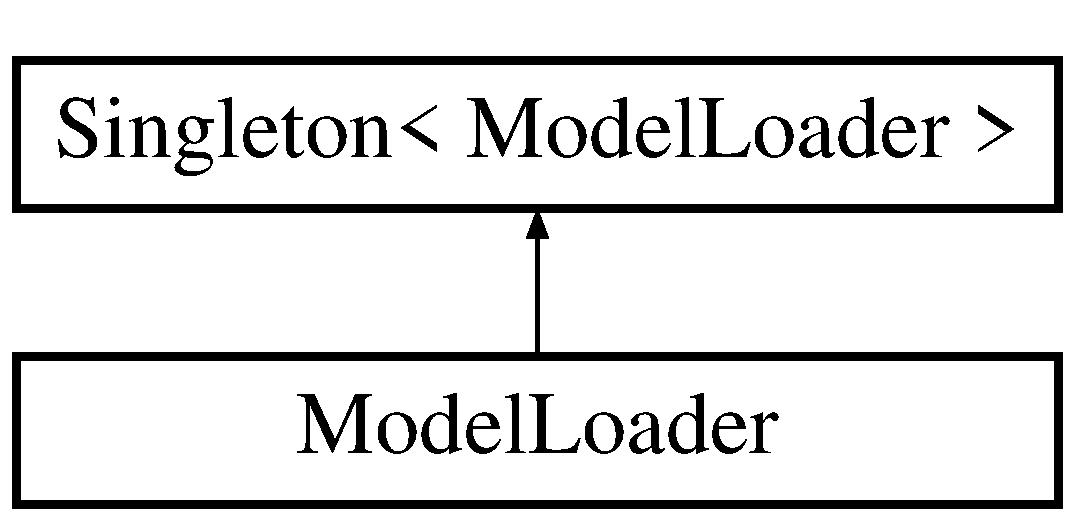
\includegraphics[height=2cm]{classModelLoader}
\end{center}
\end{figure}
\subsection*{Classes}
\begin{DoxyCompactItemize}
\item 
struct \hyperlink{structModelLoader_1_1Model}{Model}
\item 
struct \hyperlink{structModelLoader_1_1point}{point}
\end{DoxyCompactItemize}
\subsection*{Public Member Functions}
\begin{DoxyCompactItemize}
\item 
\hypertarget{classModelLoader_ac14dc611ee3ec0f7a20294ea9509fb10}{
void {\bfseries CreateCubeModel} (const std::string \&gameModelName)}
\label{classModelLoader_ac14dc611ee3ec0f7a20294ea9509fb10}

\item 
\hypertarget{classModelLoader_a86c83b98085243935a6a0de0785c7512}{
void {\bfseries CreateCubeModel2} (const std::string \&gameModelName)}
\label{classModelLoader_a86c83b98085243935a6a0de0785c7512}

\item 
\hypertarget{classModelLoader_ae45b20a6326655a86b61c43a8bec2d17}{
void {\bfseries CreateGrid} (const std::string \&gameModelName)}
\label{classModelLoader_ae45b20a6326655a86b61c43a8bec2d17}

\item 
\hypertarget{classModelLoader_ae807caa16c2e2b1c87eeebb344ba7ebb}{
void {\bfseries createVBOgrid} (const std::string \&gameModelName)}
\label{classModelLoader_ae807caa16c2e2b1c87eeebb344ba7ebb}

\item 
\hypertarget{classModelLoader_aa85f00738360bfc64f31f2e11c4efc58}{
void {\bfseries DeleteModel} (const std::string \&gameModelName)}
\label{classModelLoader_aa85f00738360bfc64f31f2e11c4efc58}

\item 
\hypertarget{classModelLoader_a1e37e94c952b4157ff071146bfee927a}{
unsigned int {\bfseries GetModel} (const std::string \&gameModelName)}
\label{classModelLoader_a1e37e94c952b4157ff071146bfee927a}

\item 
\hypertarget{classModelLoader_a522ddc775b7b60f89bc36242e806cbf0}{
glm::vec3 {\bfseries GetPosition} ()}
\label{classModelLoader_a522ddc775b7b60f89bc36242e806cbf0}

\item 
\hypertarget{classModelLoader_ab57ba52335d4efd8b55d843d3801ca3c}{
void {\bfseries SetPosition} (glm::vec3 \_\-position)}
\label{classModelLoader_ab57ba52335d4efd8b55d843d3801ca3c}

\item 
\hypertarget{classModelLoader_a5bf2312dc46e142f1877739dfcc756e8}{
glm::vec3 {\bfseries GetRotation} ()}
\label{classModelLoader_a5bf2312dc46e142f1877739dfcc756e8}

\item 
\hypertarget{classModelLoader_a428ef884d300bc2b2d0706ad5b4198ca}{
void {\bfseries SetRotation} (glm::vec3 \_\-rotation)}
\label{classModelLoader_a428ef884d300bc2b2d0706ad5b4198ca}

\item 
\hypertarget{classModelLoader_afc0ecdf73f6c85752c9a690e38599b34}{
glm::vec3 {\bfseries GetScale} ()}
\label{classModelLoader_afc0ecdf73f6c85752c9a690e38599b34}

\item 
\hypertarget{classModelLoader_a96793c518f235d03349f642ad0aaebc1}{
void {\bfseries SetScale} (glm::vec3 \_\-scale)}
\label{classModelLoader_a96793c518f235d03349f642ad0aaebc1}

\item 
\hypertarget{classModelLoader_a50486cfb738a0f1431b8de2dad3f00ff}{
void {\bfseries SetViewMatrix} (glm::mat4 \_\-viewMatrix)}
\label{classModelLoader_a50486cfb738a0f1431b8de2dad3f00ff}

\item 
\hypertarget{classModelLoader_a9d3d71a699f08533e95a8af4530eaa04}{
glm::mat4 {\bfseries GetViewMatrix} ()}
\label{classModelLoader_a9d3d71a699f08533e95a8af4530eaa04}

\item 
\hypertarget{classModelLoader_a5a7bcbfb9d6c71c1ea58b150be4b991c}{
void {\bfseries SetProjectionMatrix} (glm::mat4 \_\-projectionMatrix)}
\label{classModelLoader_a5a7bcbfb9d6c71c1ea58b150be4b991c}

\item 
\hypertarget{classModelLoader_aa4f1ba034a863e7f9ca8628360e2384a}{
glm::mat4 {\bfseries GetProjectionMatrix} ()}
\label{classModelLoader_aa4f1ba034a863e7f9ca8628360e2384a}

\end{DoxyCompactItemize}
\subsection*{Public Attributes}
\begin{DoxyCompactItemize}
\item 
\hypertarget{classModelLoader_aa3eb17f659b30e28874112f08f676e18}{
GLint {\bfseries posAttrib} = glGetAttribLocation(m\_\-shaderProgramId, \char`\"{}in\_\-position\char`\"{})}
\label{classModelLoader_aa3eb17f659b30e28874112f08f676e18}

\item 
\hypertarget{classModelLoader_a52a0d4556d91017494e44259692c48d3}{
GLint {\bfseries colAttrib} = glGetAttribLocation(m\_\-shaderProgramId, \char`\"{}in\_\-color\char`\"{})}
\label{classModelLoader_a52a0d4556d91017494e44259692c48d3}

\item 
\hypertarget{classModelLoader_aada21d4b482693f92d503a9beab03abb}{
GLint {\bfseries texAttrib} = glGetAttribLocation(m\_\-shaderProgramId, \char`\"{}in\_\-uv\char`\"{})}
\label{classModelLoader_aada21d4b482693f92d503a9beab03abb}

\item 
\hypertarget{classModelLoader_a590d418ab85aa4654ef94b25eada91d0}{
unsigned int {\bfseries Gridvbo}}
\label{classModelLoader_a590d418ab85aa4654ef94b25eada91d0}

\item 
\hypertarget{classModelLoader_a494e2a0ce1c438005a78611fedeca593}{
GLuint {\bfseries m\_\-shaderProgramId}}
\label{classModelLoader_a494e2a0ce1c438005a78611fedeca593}

\end{DoxyCompactItemize}
\subsection*{Friends}
\begin{DoxyCompactItemize}
\item 
\hypertarget{classModelLoader_af3bfa18f3438adae73421a11b6401066}{
class \hyperlink{classModelLoader_af3bfa18f3438adae73421a11b6401066}{Singleton$<$ ModelLoader $>$}}
\label{classModelLoader_af3bfa18f3438adae73421a11b6401066}

\end{DoxyCompactItemize}


The documentation for this class was generated from the following files:\begin{DoxyCompactItemize}
\item 
ModelLoader.h\item 
ModelLoader.cpp\end{DoxyCompactItemize}

\hypertarget{structModelLoader_1_1point}{
\section{ModelLoader::point Struct Reference}
\label{structModelLoader_1_1point}\index{ModelLoader::point@{ModelLoader::point}}
}
\subsection*{Public Attributes}
\begin{DoxyCompactItemize}
\item 
\hypertarget{structModelLoader_1_1point_a9181ecbd09f8ac975b0979820ca1764f}{
GLfloat {\bfseries x}}
\label{structModelLoader_1_1point_a9181ecbd09f8ac975b0979820ca1764f}

\item 
\hypertarget{structModelLoader_1_1point_ad698d96b1ffc1ec5995d27bc06002716}{
GLfloat {\bfseries y}}
\label{structModelLoader_1_1point_ad698d96b1ffc1ec5995d27bc06002716}

\item 
\hypertarget{structModelLoader_1_1point_a26c0891fc203a53111bb3df17e654b9a}{
GLfloat {\bfseries z}}
\label{structModelLoader_1_1point_a26c0891fc203a53111bb3df17e654b9a}

\end{DoxyCompactItemize}


The documentation for this struct was generated from the following file:\begin{DoxyCompactItemize}
\item 
ModelLoader.h\end{DoxyCompactItemize}

\hypertarget{classShader}{
\section{Shader Class Reference}
\label{classShader}\index{Shader@{Shader}}
}
\subsection*{Public Member Functions}
\begin{DoxyCompactItemize}
\item 
\hypertarget{classShader_aab6796612c50cc11ad6ebf31c4c4386d}{
{\bfseries Shader} (const std::string \&filename)}
\label{classShader_aab6796612c50cc11ad6ebf31c4c4386d}

\item 
\hypertarget{classShader_a6f6e280a343d6c7662909f7dfbc89ad9}{
void {\bfseries bind} ()}
\label{classShader_a6f6e280a343d6c7662909f7dfbc89ad9}

\item 
\hypertarget{classShader_a51373dbc46459f823c38f987b13f3975}{
void {\bfseries InitShaders} (std::string strVertex, std::string strFragment)}
\label{classShader_a51373dbc46459f823c38f987b13f3975}

\item 
\hypertarget{classShader_ab54c6fe63a0961380132be979f00a791}{
void {\bfseries Release} ()}
\label{classShader_ab54c6fe63a0961380132be979f00a791}

\item 
\hypertarget{classShader_a97bac997e4e8ff3ea8f072e09110fbff}{
GLuint {\bfseries getVertexShaderId} ()}
\label{classShader_a97bac997e4e8ff3ea8f072e09110fbff}

\item 
\hypertarget{classShader_a8eadc6215cec4c15d283783231f60318}{
GLuint {\bfseries getFragmaneShaderId} ()}
\label{classShader_a8eadc6215cec4c15d283783231f60318}

\item 
\hypertarget{classShader_a4112f1b765a232e472d2c3f82d036371}{
GLuint {\bfseries getProgramShaderId} ()}
\label{classShader_a4112f1b765a232e472d2c3f82d036371}

\end{DoxyCompactItemize}
\subsection*{Static Public Member Functions}
\begin{DoxyCompactItemize}
\item 
\hypertarget{classShader_a9645692b6d18b34c8094c329a9a4d343}{
static std::string {\bfseries LoadShader} (const std::string \&fileName)}
\label{classShader_a9645692b6d18b34c8094c329a9a4d343}

\end{DoxyCompactItemize}


The documentation for this class was generated from the following files:\begin{DoxyCompactItemize}
\item 
shader.h\item 
shader.cpp\end{DoxyCompactItemize}

\hypertarget{classSingleton}{
\section{Singleton$<$ T $>$ Class Template Reference}
\label{classSingleton}\index{Singleton@{Singleton}}
}
\subsection*{Static Public Member Functions}
\begin{DoxyCompactItemize}
\item 
\hypertarget{classSingleton_a57cb3b89f16fc5926bebf3b07b627b03}{
static T $\ast$ {\bfseries Singleton} (int shaderProgramId)}
\label{classSingleton_a57cb3b89f16fc5926bebf3b07b627b03}

\item 
\hypertarget{classSingleton_a1d1165bbf5ba233fe8fa7198685fce43}{
static void {\bfseries DestroySingleton} ()}
\label{classSingleton_a1d1165bbf5ba233fe8fa7198685fce43}

\end{DoxyCompactItemize}
\subsection*{Protected Member Functions}
\begin{DoxyCompactItemize}
\item 
\hypertarget{classSingleton_a52d4e99fde1c7240d0a622ec7ddcda04}{
{\bfseries Singleton} (const \hyperlink{classSingleton}{Singleton} \&other)}
\label{classSingleton_a52d4e99fde1c7240d0a622ec7ddcda04}

\item 
\hypertarget{classSingleton_a0d67df9f1bce51f33c48eab587a91890}{
\hyperlink{classSingleton}{Singleton} \& {\bfseries operator=} (const \hyperlink{classSingleton}{Singleton} \&other)}
\label{classSingleton_a0d67df9f1bce51f33c48eab587a91890}

\end{DoxyCompactItemize}
\subsection*{Static Protected Attributes}
\begin{DoxyCompactItemize}
\item 
\hypertarget{classSingleton_a77987e85742da3505825c3195ed7c8a6}{
static T $\ast$ {\bfseries m\_\-instance} = NULL}
\label{classSingleton_a77987e85742da3505825c3195ed7c8a6}

\end{DoxyCompactItemize}
\subsubsection*{template$<$class T$>$ class Singleton$<$ T $>$}



The documentation for this class was generated from the following file:\begin{DoxyCompactItemize}
\item 
singleton.h\end{DoxyCompactItemize}

\hypertarget{structVertexStructure}{
\section{VertexStructure Struct Reference}
\label{structVertexStructure}\index{VertexStructure@{VertexStructure}}
}
\subsection*{Public Member Functions}
\begin{DoxyCompactItemize}
\item 
\hypertarget{structVertexStructure_a9c4c269cd69720c0043717b9bbb23696}{
{\bfseries VertexStructure} (const glm::vec3 \&pos, const glm::vec4 \&col, const glm::vec2 \&tex)}
\label{structVertexStructure_a9c4c269cd69720c0043717b9bbb23696}

\end{DoxyCompactItemize}
\subsection*{Public Attributes}
\begin{DoxyCompactItemize}
\item 
\hypertarget{structVertexStructure_a404fdf9024416b6f525f3dafcbac2b02}{
glm::vec3 {\bfseries position}}
\label{structVertexStructure_a404fdf9024416b6f525f3dafcbac2b02}

\item 
\hypertarget{structVertexStructure_a9095e44220ac792f9c9cbc7ebaa6216c}{
glm::vec4 {\bfseries color}}
\label{structVertexStructure_a9095e44220ac792f9c9cbc7ebaa6216c}

\item 
\hypertarget{structVertexStructure_a8437741620daad43e3052c614d1c56f1}{
glm::vec2 {\bfseries textureUV}}
\label{structVertexStructure_a8437741620daad43e3052c614d1c56f1}

\end{DoxyCompactItemize}


The documentation for this struct was generated from the following file:\begin{DoxyCompactItemize}
\item 
Vertexformat.h\end{DoxyCompactItemize}

\printindex
\end{document}
